% =====================================================================
%  MICAI 2027 Submission -- DOUBLE-BLIND REVIEW VERSION
%  Springer LNCS / LNAI format (llncs.cls)
%
%  Blocks that differ between review and camera-ready are marked
%  "% >>> REVIEW:" / "% >>> CAMERA-READY:". For the anonymous PDF keep
%  the REVIEW blocks; for camera-ready swap to the CAMERA-READY blocks
%  (author block, code/data availability URLs, acknowledgments, named
%  institutions in the ethics statement).
%
%  OVERLEAF: upload llncs.cls and the Figures/ folder (bibliography is inline).
%  Compiler = pdfLaTeX. Run pdfLaTeX x2 (inline thebibliography; no bibtex step).
%  Do NOT load geometry / override margins (Springer rejects it).
%  Figures are generated by make_paper_figures.py (`make paper-figures`).
% =====================================================================
\documentclass[runningheads]{llncs}
\AtBeginDocument{\pdfpagewidth=210mm \pdfpageheight=297mm}

\usepackage[T1]{fontenc}
\usepackage[utf8]{inputenc}
\usepackage[english]{babel}
\usepackage{graphicx}
\usepackage{booktabs}
\usepackage{amsmath}
\usepackage{amssymb}
\usepackage{array}
\usepackage{xcolor}
\usepackage{hyperref}
\renewcommand\UrlFont{\color{black}\rmfamily}
\urlstyle{rm}
\graphicspath{{Figures/}}

\newcommand{\smape}{sMAPE}
\newcommand{\mase}{MASE}
\newcommand{\mae}{MAE}
\newcommand{\rmse}{RMSE}

\begin{document}

\title{A Public Multi-Series Panel and a Leakage-Free Prospective
Evaluation Protocol for Forecasting U.S. Visa Bulletin Priority Dates}
\titlerunning{Forecasting U.S. Visa Bulletin Priority Dates}

% >>> REVIEW:
\author{Anonymous Author(s)}
\authorrunning{Anonymous}
\institute{Affiliations withheld for double-blind review}
% >>> CAMERA-READY (uncomment for the final version; comment out the REVIEW block above):
% \author{Javier A. Rebull Saucedo\inst{1}\orcidID{0000-0000-0000-0000} \and
%   Vicente Garc\'ia Jim\'enez\inst{1}\orcidID{0000-0000-0000-0000}}
% \authorrunning{J. A. Rebull and V. Garc\'ia}
% \institute{Maestr\'ia en Inteligencia Artificial y Anal\'itica de Datos (MIAAD),
%   Universidad Aut\'onoma de Ciudad Ju\'arez, Ciudad Ju\'arez, Chihuahua, M\'exico \\
%   \email{al263483@alumnos.uacj.mx}, \email{vicente.jimenez@uacj.mx}}
% (Fill in real ORCIDs before submission. Requires \usepackage{orcidlink} or the
%  llncs \orcidID macro; remove \orcidID if unavailable.)

\maketitle

\begin{abstract}
The U.S. Department of State publishes the monthly \emph{Visa Bulletin}, whose
per-country, per-category priority-date cutoffs govern the immigrant-visa queue
for millions of applicants, yet no open, systematically evaluated forecasting
resource exists. We contribute (i)~a public, audited multi-series panel of
priority dates (194 structural series; country $\times$ category $\times$ table
$\times$ month; December~2001--2026), (ii)~a per-series benchmark of forecasting
models under leakage-free expanding walk-forward, and (iii)~a \emph{prospective}
evaluation protocol that scores forecasts \emph{frozen} at a dated origin against
the cutoffs actually published afterwards. On 2{,}944 prospectively scored
forecasts the mean absolute error is 146~days and the scaled error (MASE) 0.345,
degrading smoothly from one to twelve months ahead yet remaining below the
seasonal-naïve baseline (MASE~$<1$) at every horizon. 95\% prediction intervals
attain 0.92 empirical coverage (under the nominal level, reported as such).
Consistent with the M4/M5 competitions, well-tuned parsimonious statistics are hard
to beat: per series, ETS and Theta form the model confidence set, and a tuned
Auto-ARIMA is a strong baseline. The globally trained deep model only \emph{matches}
them on the longer Final-Action-Dates series; it retains a modest ($\approx$11\% in
the mean) edge on the shorter Dates-for-Filing series, but that edge is sensitive to
the aggregation and rests on a small effective sample. We release the panel, code,
and a reproducible evaluation pipeline.
\keywords{Time-series forecasting \and Prospective evaluation \and Conformal
prediction \and Open dataset \and Immigration analytics \and Reproducibility}
\end{abstract}

% =====================================================================
\section{Introduction}
\label{sec:intro}

The U.S. \emph{Visa Bulletin} publishes, each month, the \emph{priority-date}
cutoffs that determine which immigrant-visa petitions may advance, broken down by
country (or chargeability area), preference category, and one of two tables
---Final Action Dates (FAD) and Dates for Filing (DFF). These cutoffs move
non-monotonically: they advance, stall, or \emph{retrogress} as annual quotas are
consumed, producing shocks that matter to millions of applicants. Despite three
decades of public data, we found no open, systematically evaluated forecasting
resource for these series, and---critically---no evaluation that reports how a
forecast \emph{frozen today} performs against what is \emph{actually published}
later.

This paper addresses that gap with three contributions:
\begin{enumerate}
  \item A \textbf{public, audited multi-series panel} $y_{p,c,b,t}$ (priority-date
  days since a fixed epoch) covering 194 structural series and 27{,}289
  observations (Sec.~\ref{sec:data}), built from State-Department HTML frozen for
  reproducibility, with an explicit Current/Final/Unavailable regime annotation.
  \item A \textbf{per-series forecasting benchmark} under leakage-free expanding
  walk-forward (Sec.~\ref{sec:eval}), comparing parsimonious statistical models,
  gradient-boosted trees, and globally trained neural models.
  \item A \textbf{prospective evaluation protocol} (Sec.~\ref{sec:prospective})
  that archives each forecast with its origin and scores it against subsequently
  published cutoffs---the honest, out-of-sample measure of real-world accuracy,
  reported alongside (not in place of) the retrospective walk-forward signal.
\end{enumerate}
We deliberately frame this as an \emph{application} contribution: the dataset and
the prospective protocol, not a new model. An auditable web interface to the
forecasts accompanies the artifacts (Sec.~\ref{sec:ethics}) but is not part of
the scientific claim.

% =====================================================================
\section{Related Work}
\label{sec:related}

\paragraph{Global vs.\ local forecasting.} The M4/M5 competitions established that
simple statistical methods are hard to beat and that complexity must earn its
keep~\cite{makridakis2020,makridakis2022}; Montero-Manso and Hyndman~\cite{montero2021}
formalize when a single \emph{global} model trained across many series outperforms
per-series \emph{local} models. Our result (Sec.~\ref{sec:results}) is consistent
with this literature and with the M4/M5 ``simple-beats-complex'' finding: global deep
models match the tuned statistical baselines on one table and hold only a modest edge
on the other. The Monash archive~\cite{godahewa2021} popularized
standardized multi-series benchmarking, which we follow.

\paragraph{Models and intervals.} We compare exponential smoothing and Theta,
(S)ARIMA, gradient-boosted trees, and global neural models~\cite{salinas2020,
oreshkin2020,nie2023}; prediction intervals use split conformal
prediction~\cite{vovk2005,romano2019}, which gives finite-sample coverage under
exchangeability for one-step forecasts. Forecast accuracy is summarized with the
scaled error MASE~\cite{hyndman2006} and compared with the Diebold--Mariano test
under the Harvey--Leybourne--Newbold small-sample correction~\cite{diebold1995,harvey1997};
multiple-model rankings use Friedman with a Nemenyi post-hoc~\cite{demsar2006}. The
pipeline follows the CRISP-DM process model~\cite{chapman2000}.

\paragraph{Immigration analytics.} Public reporting documents multi-year
retrogressions in employment categories for demand-heavy countries~\cite{bier2023};
to our knowledge no peer-reviewed, openly evaluated forecasting study of the Visa
Bulletin panel exists, which motivates the dataset contribution.

% =====================================================================
\section{Materials and Methods}
\label{sec:methods}

\subsection{Data Characterization}
\label{sec:data}

We parse the monthly Visa Bulletin into a tidy panel $y_{p,c,b,t}$ indexed by
country/area $p$, category $c$, table $b\in\{\mathrm{FAD},\mathrm{DFF}\}$, and
bulletin month $t$. The dependent variable is \texttt{days\_since\_base}, the
priority-date cutoff expressed as days since a fixed epoch ($t_0=$~1~Jan~1975, which
precedes every observed priority date). Each cell carries a regime label
$e\in\{C,F,U\}$: \emph{Current} (no backlog), \emph{Final} (a specific cutoff
date), or \emph{Unavailable}. \textbf{We model only $e=F$ cells}; $C$ and $U$ are
descriptive annotations, not forecasting targets, and the system does not predict
regime transitions---an explicit scope limitation. To prevent target leakage,
\texttt{days\_since\_base} is non-null \emph{if and only if} $e=F$, an invariant
enforced by database constraints.

The homogeneous monthly series the pipeline reconstructs spans
\textbf{December~2001--2026} ($\approx$290 months); FAD have been published since
1992, but the continuous machine-readable series begins in 2001 (the 1992--2001
period is reserved for future archival integration). The panel contains
\textbf{194 structural series and 27{,}289 observations}; of these, 136 series have
at least one $F$ observation and \textbf{74 have $\geq$84 $F$ observations}
(initial window plus hold-out) and are thus fully evaluable. We report results on
the evaluable subset and never claim to ``model 194 series.'' Raw HTML is frozen in
object storage so the panel rebuilds byte-for-byte offline. Diversity-Visa data are
maintained as a \emph{separate} rank-valued fact, not a predictive target.

\subsection{Models}
\label{sec:models}

Behind a common interface we evaluate parsimonious statistical models (seasonal
naïve, ETS, Theta, ARIMA, SARIMA), gradient-boosted trees (XGBoost, LightGBM,
CatBoost) on differenced targets with calendar covariates, and globally trained
neural models (BiTCN, N-HiTS, PatchTST, TiDE) with per-series normalization. The
seasonal-naïve forecaster, which also defines the MASE denominator, is reported as
an explicit baseline row, not only as a scaling factor.

\subsection{Evaluation Protocol}
\label{sec:eval}

\paragraph{Walk-forward.} Models are evaluated with expanding-window walk-forward
(initial window 60 months for FAD / 36 for DFF; step one month; final 24 months
held out and never used for selection). At each origin the forecast uses only the
past. FAD and DFF are evaluated separately and never mixed.

\paragraph{Leakage prevention.} (i)~The expanding window references only pre-origin
observations; tree-model lags and rolling statistics are computed strictly before
the origin. (ii)~Multi-step forecasts roll out recursively, filling future lags with
\emph{predictions}, never observed future values; error accumulation is reported as
a limitation. (iii)~The MASE denominator (in-sample seasonal-naïve error) is
computed only on data preceding the origin, aligned by date to remain robust to
$C/U$ gaps. (iv)~For the prospective protocol, the forecast and its calibration are
\emph{frozen at a dated origin that precedes} the bulletins against which they are
scored (Sec.~\ref{sec:prospective}).

\paragraph{Metrics and significance.} Point accuracy uses MASE (primary, scale-free
across heterogeneous series), MAE, RMSE, and \smape. Pairwise out-of-sample
comparisons use Diebold--Mariano with the HLN small-sample
correction~\cite{diebold1995,harvey1997}, framing non-rejection as
\emph{insufficient evidence to separate}, not equivalence; multi-model rankings use
Friedman--Nemenyi~\cite{demsar2006}.

\paragraph{Prediction intervals.} One-step 95\% intervals are obtained by split
conformal calibration on the hold-out residuals~\cite{vovk2005}, which guarantees
finite-sample coverage \emph{at one step}. For multi-step intervals we widen the
one-step half-width by $\sqrt{h}$; \textbf{this is a heuristic and does not transfer
the conformal guarantee to $h>1$}---we therefore report \emph{empirical} multi-step
coverage (Sec.~\ref{sec:prospective}) rather than claiming a guarantee. The 80\%
band width is calibrated as a fixed multiple of the 95\% half-width, estimated on a
\emph{disjoint} set of vintages and validated on held-out vintages so the reported
80\% coverage is out-of-sample.

\paragraph{Deployed configuration.} For the public-facing forecasts we deploy a
parsimonious production configuration---the median of \{Theta, ETS, SARIMA\} for FAD
and SARIMA for DFF---chosen for determinism, CPU reproducibility, and robustness;
on FAD this trades a statistically insignificant gap against the deep models for
operational simplicity (Sec.~\ref{sec:results}). The prospective evaluation scores
the model \emph{actually deployed}.

% =====================================================================
\section{Results}
\label{sec:results}

\paragraph{Per-series benchmark.} Under walk-forward, parsimony is hard to beat per
series: ETS/Theta reach a hold-out MASE of $\approx$0.117 on family FAD and
gradient-boosted trees are competitive on DFF. Locally trained deep models fail on
the short individual series. Trained \emph{globally} (across series, on differenced
and per-series-normalized targets, with hyper-parameter search), deep models recover:
on FAD an AutoBiTCN configuration reaches mean MASE $0.112$, a seed confidence
interval that contains the ETS/Theta value of $0.117$---a \emph{tie}; a per-table
Diebold--Mariano test finds no significant FAD separation. On DFF, BiTCN reaches mean
MASE $0.090$, ahead of the best classical baseline; the size of that lead and its
robustness are examined with a tuned Auto-ARIMA below. We emphasize that this
hold-out MASE is a \emph{selection signal}, not a prediction of live accuracy; the
honest out-of-sample number is three times larger (Sec.~\ref{sec:prospective}).

\paragraph{Statistical significance.} A Friedman test over the per-series hold-out
MASE of the local pool rejects equal performance in both tables ($p<10^{-28}$;
Table~\ref{tab:significance}). We deduplicate the cross-sectional pseudo-replicates
first---the worldwide cut-off is repeated identically across several countries, so the
25 family cells reduce to about 14--15 \emph{distinct} series---which is why the DFF
test runs on fewer effective series. With a Nemenyi post-hoc (Fig.~\ref{fig:cd}) and a
90\% Model Confidence Set~\cite{demsar2006}, the \emph{only} models that survive in
both tables are \textbf{ETS and Theta}; SARIMA, the gradient-boosted trees, and all
locally trained deep models are excluded. The globally trained deep model edges the
SARIMA baseline on FAD (Diebold--Mariano, $p\approx0.01$), but the result is \emph{not
robust} to which near-tied deep model is designated (an alternative gives $p\approx0.23$)
and the deep model does not enter the $\{$ETS, Theta$\}$ confidence set---consistent with
our framing of FAD as a tie. On DFF the \emph{global} deep model (a separate training
regime) reaches MASE~0.090, on par with the best classical baselines rather than ahead of
them, and its edge is likewise not robust to deep-model choice ($p$ from 0.007 to 0.08;
see the tuned-baseline paragraph below).

\begin{table}[t]\centering\footnotesize
\caption{Friedman--Nemenyi over the per-series hold-out MASE of the model pool.
Lower mean rank is better; $^\star$ marks membership in the 90\% Model Confidence
Set. The Friedman $p$ rejects equal performance; only ETS and Theta enter the MCS.}
\label{tab:significance}
\begin{tabular}{llll}
\toprule
Table & \#models & Friedman $p$ & Top-6 by mean rank (MCS $^\star$) \\
\midrule
FAD & 20 & $3{\times}10^{-74}$ & ets (2.1$^\star$), theta (2.3$^\star$), arima (3.9), rlinear (4.8), nlinear (4.9), catboost (6.6) \\
DFF & 18 & $1{\times}10^{-29}$ & ets (2.9$^\star$), catboost (3.9), theta (4.3$^\star$), xgboost (4.6), rlinear (5.6), nlinear (5.8) \\
\bottomrule
\end{tabular}
\end{table}

\begin{figure}[t]
\centering
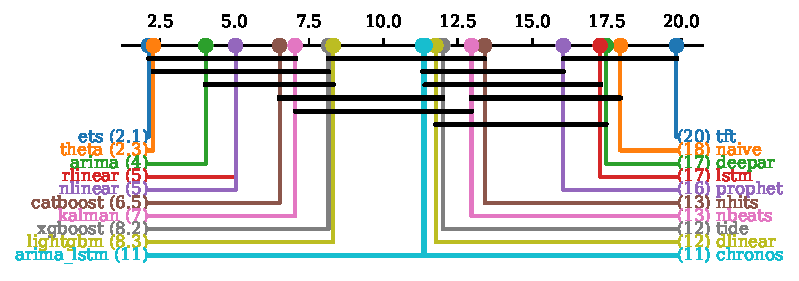
\includegraphics[width=0.92\textwidth]{fig_cd_diagram.pdf}
% ALT-TEXT: Demsar critical-difference diagram for the 20 FAD models; ETS (2.1) and
% Theta (2.3) at the best end, connected bars show statistically tied groups.
\caption{Critical-difference diagram (FAD): mean ranks of the model pool with
Nemenyi-connected groups. ETS and Theta lead and form the confidence set.}
\label{fig:cd}
\end{figure}

\paragraph{Tuned classical baseline.} To guard against beating weak baselines, we
add an order-selected Auto-ARIMA (AICc grid search on the pre-hold-out window, same
walk-forward). On FAD its mean MASE is 0.161 (median 0.135)---\emph{worse} than ETS
(0.119) and Theta (0.118), which confirms them as the FAD champions and the deep
model as their tie. On DFF, Auto-ARIMA is the strongest classical (mean 0.101, median
0.086), so the deep model's DFF lead, originally stated against gradient-boosted
trees ($\approx$0.116), narrows to $\approx$11\% against this tuned baseline
(BiTCN~0.090 vs.\ 0.101 in the mean). That lead is moreover \emph{aggregation
sensitive}: under the median, Auto-ARIMA (0.086) ties BiTCN (0.090), and the
$\approx$25 DFF family series collapse to only $\approx$14 distinct series once the
shared-world-cutoff pseudo-replication is removed (Sec.~\ref{sec:discussion}). We
therefore present the DFF result as a \emph{modest, fragile} edge on a small
effective sample rather than a decisive win---in line with the M4/M5 lesson that
well-tuned parsimony is hard to beat.
% =====================================================================
\section{Out-of-Sample Prospective Evaluation}
\label{sec:prospective}

Walk-forward repeatedly predicts \emph{already known} months; it measures
selection, not the real-world quality of a forecast issued today. We therefore
\emph{freeze} each forecast with its origin month in an append-only ledger and,
as bulletins are published, score it against the cutoff actually observed.

\paragraph{Aggregate behavior.} Over \textbf{2{,}944} prospectively scored
forecasts (Table~\ref{tab:prospective}), the mean absolute error is
\textbf{146~days} and MASE \textbf{0.345}. Accuracy degrades smoothly with the
horizon (Fig.~\ref{fig:prospective} (left)): from $\approx$20~days / MASE~0.05 at one month to
$\approx$351~days / MASE~0.75 at twelve months. Crucially, MASE stays
\emph{below~1} at every horizon---the forecasts beat the seasonal-naïve baseline
even a year out. The retrospective hold-out MASE (0.117) and the prospective MASE
(0.345) differ by $\approx$3$\times$; this gap is expected (repeated one-step vs.\
genuine one-to-twelve-step extrapolation through retrogression shocks) and is
disclosed rather than hidden.

\paragraph{Calibration.} The 95\% intervals attain \textbf{0.92} empirical coverage
overall (Fig.~\ref{fig:prospective} (right))---slightly \emph{below} the nominal level,
which we report as honest under-coverage rather than tuning to appear calibrated.
The disjoint-split--calibrated 80\% band attains 0.81 out-of-sample coverage. Per
table, FAD intervals are better calibrated (0.95) than the shorter, shock-prone DFF
series (0.89).

\paragraph{Scope of the prospective set.} The ledger lists ten origin vintages, but
only three recent origins (2024-07, 2025-01, 2025-07) contribute scored forecasts;
the others originate from series whose last $F$ observation predates the window and
contribute none. We report the effective vintage count explicitly. These vintages
are \emph{leakage-free backfills}---each model and its calibration are truncated to
the origin---but a backfill is \emph{not} identical to having served the forecast
in real time; going forward the ledger accumulates genuinely live vintages.

\begin{table}[t]
\centering
\caption{Prospective evaluation (frozen forecasts vs.\ published cutoffs).
Coverage is empirical; nominal levels are 0.80 and 0.95. The 80\% band is
calibrated on a disjoint vintage split; ``cov$_{80}$ held-out'' is its
out-of-sample coverage.}
\label{tab:prospective}
\footnotesize
\begin{tabular}{lrrrrr}
\toprule
Subset & $n$ & MAE (days) & MASE & cov$_{95}$ & cov$_{80}$ \\
\midrule
FAD            & 1{,}704 & 156.0 & 0.319 & 0.949 & 0.833 \\
DFF            & 1{,}240 & 131.5 & 0.381 & 0.890 & 0.765 \\
\midrule
\textbf{Overall} & \textbf{2{,}944} & \textbf{145.7} & \textbf{0.345} & \textbf{0.924} & 0.804 \\
\multicolumn{6}{l}{\footnotesize cov$_{80}$ held-out (out-of-sample) $=0.81$.} \\
\bottomrule
\end{tabular}
\end{table}

\begin{figure}[t]
\centering
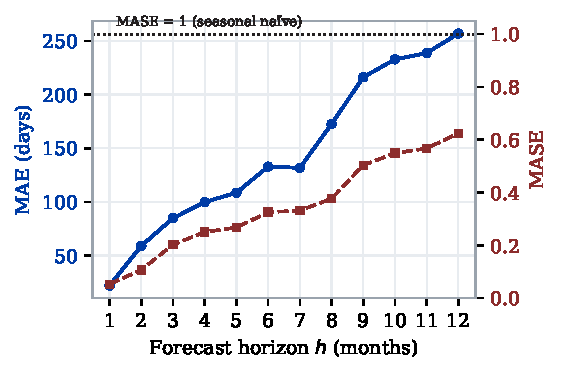
\includegraphics[width=0.49\textwidth]{fig_prospective_horizon.pdf}
\hfill
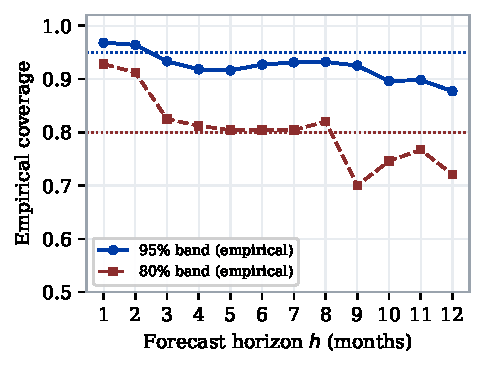
\includegraphics[width=0.49\textwidth]{fig_calibration.pdf}
% ALT-TEXT: left, MAE in days (left axis) and MASE (right axis) rising with the
% forecast horizon 1-12 months, MASE staying below the dotted naive=1 line; right,
% empirical 95% and 80% coverage vs horizon against dotted nominal references.
\caption{\textbf{Left:} prospective error vs.\ horizon; MASE remains below the
seasonal-naïve reference (MASE$=1$) at all horizons. \textbf{Right:} empirical
interval coverage vs.\ horizon, with nominal references.}
\label{fig:prospective}
\end{figure}

\begin{figure}[t]
\centering
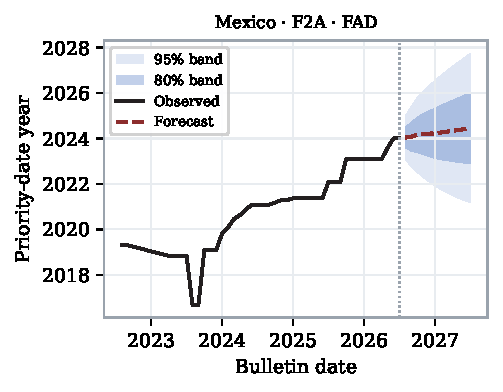
\includegraphics[width=0.6\textwidth]{fig_fanchart.pdf}
% ALT-TEXT: observed priority-date year for Mexico F2A FAD over the last six years,
% a vertical "today" marker, and a dashed 12-month forecast with nested 80/95% bands.
\caption{Representative frozen forecast (Mexico, F2A, FAD): observed history, a
dated origin (vertical marker), and the 12-month forecast with 80\%/95\% bands.}
\label{fig:fan}
\end{figure}

% =====================================================================
\section{Discussion}
\label{sec:discussion}

The central, defensible message is conservative, in the M4/M5 tradition: on this
panel a well-tuned parsimonious suite (ETS, Theta, order-selected Auto-ARIMA) is hard
to beat. The globally trained deep model matches it on FAD and holds only a modest,
aggregation-sensitive edge on DFF ($\approx$11\% in the mean over a small effective
sample); neither gradient-boosted trees nor deep learning dominate the tuned
statistical baselines. The prospective protocol additionally exposes a $3\times$ optimism in
the retrospective hold-out number---a discrepancy that any single-split benchmark
hides and that practitioners deploying such systems must know.

\paragraph{Threats to validity.} (1)~Multi-step intervals use a $\sqrt{h}$ heuristic
without a multi-step coverage guarantee; observed 95\% coverage falls from
$\approx$0.97 to $\approx$0.88 across horizons. (2)~The effective prospective sample
is three recent vintages; broader temporal coverage will accrue as live vintages
accumulate. (3)~\textbf{Pseudo-replication is severe for DFF}: when a world cutoff is
shared, the ``All-Chargeability'' row is identical to the per-country rows, so the
$\approx$25 DFF family series reduce to only $\approx$5--7 distinct series; DFF
conclusions therefore rest on a small effective sample and pairwise DFF comparisons
should be read as indicative. (4)~Deep results depend on a single accelerator and a
fixed seed set. (5)~Some statistical models converge only on series subsets
(survivorship), disclosed where aggregates are averaged.

% =====================================================================
\section{Conclusions}
\label{sec:conclusions}

We release an open, audited multi-series panel of U.S. Visa Bulletin priority dates
and a leakage-free \emph{prospective} evaluation protocol that scores frozen
forecasts against subsequently published cutoffs. The honest out-of-sample accuracy
(MAE~146~days, MASE~0.345, beating the seasonal naïve at every horizon) and the
finding that well-tuned parsimonious models are, at worst, only modestly behind deep
learning on this panel are, we argue, more useful to practitioners than a single
optimistic hold-out number. Future work integrates the
1992--2001 archival period, models regime transitions ($C\!\leftrightarrow\!F\!\leftrightarrow\!U$),
and replaces the $\sqrt{h}$ interval heuristic with multi-step conformal methods.

% =====================================================================
\section*{Ethics and Data Availability}
\label{sec:ethics}

The data are \emph{public, aggregate} monthly Visa Bulletin tables published by the
U.S. Department of State; they contain no individual records, so no ethics-board
approval or consent was required. The source is cited with its retrieval date and
open-terms note~\cite{statedept}. The forecasts are statistical estimates and
\textbf{do not constitute legal or immigration advice}; the system explicitly does
not predict regime changes. % >>> CAMERA-READY: the panel, code, and pipeline are
% available at \url{https://github.com/UACJ-MIAAD/VisaPredictAI} and an auditable
% interface at \url{https://visapredictai.com}. (URLs withheld for review.)

% =====================================================================
\appendix
\section{Implementation and Reproducibility}
\label{sec:repro}

All experiments use Python~3.14 with pinned versions (darts, statsmodels, XGBoost,
LightGBM, CatBoost; global neural models in an isolated environment with
neuralforecast). Randomness is seeded across \texttt{random}/NumPy/Torch. Walk-forward
parameters, the F-only training mask, and the prospective ledger schema are fixed in
configuration. The prospective scorecard is regenerated end-to-end by a single
script and committed to version control with its git SHA as the durable provenance
record (experiment tracking is local-development only). Figures are produced by
\texttt{make\_paper\_figures.py} from the committed scorecard and panel.

\begin{thebibliography}{99}
\bibitem{makridakis2020} Makridakis, S., Spiliotis, E., Assimakopoulos, V.: The M4 competition. Int. J. Forecast. \textbf{36}(1), 54--74 (2020)
\bibitem{makridakis2022} Makridakis, S., Spiliotis, E., Assimakopoulos, V.: The M5 competition. Int. J. Forecast. \textbf{38}(4), 1346--1364 (2022)
\bibitem{montero2021} Montero-Manso, P., Hyndman, R.J.: Principles and algorithms for forecasting groups of time series. Int. J. Forecast. \textbf{37}(4), 1632--1653 (2021)
\bibitem{godahewa2021} Godahewa, R., Bergmeir, C., Webb, G.I., Hyndman, R.J., Montero-Manso, P.: Monash time series forecasting archive. In: NeurIPS Datasets and Benchmarks (2021)
\bibitem{salinas2020} Salinas, D., Flunkert, V., Gasthaus, J., Januschowski, T.: DeepAR. Int. J. Forecast. \textbf{36}(3), 1181--1191 (2020)
\bibitem{oreshkin2020} Oreshkin, B.N., Carpov, D., Chapados, N., Bengio, Y.: N-BEATS. In: ICLR (2020)
\bibitem{nie2023} Nie, Y., Nguyen, N.H., Sinthong, P., Kalagnanam, J.: A time series is worth 64 words: long-term forecasting with transformers (PatchTST). In: ICLR (2023)
\bibitem{vovk2005} Vovk, V., Gammerman, A., Shafer, G.: Algorithmic Learning in a Random World. Springer (2005)
\bibitem{romano2019} Romano, Y., Patterson, E., Cand\`es, E.: Conformalized quantile regression. In: NeurIPS (2019)
\bibitem{hyndman2006} Hyndman, R.J., Koehler, A.B.: Another look at measures of forecast accuracy. Int. J. Forecast. \textbf{22}(4), 679--688 (2006)
\bibitem{diebold1995} Diebold, F.X., Mariano, R.S.: Comparing predictive accuracy. J. Bus. Econ. Stat. \textbf{13}(3), 253--263 (1995)
\bibitem{harvey1997} Harvey, D., Leybourne, S., Newbold, P.: Testing the equality of prediction mean squared errors. Int. J. Forecast. \textbf{13}(2), 281--291 (1997)
\bibitem{demsar2006} Dem\v{s}ar, J.: Statistical comparisons of classifiers over multiple data sets. J. Mach. Learn. Res. \textbf{7}, 1--30 (2006)
\bibitem{chapman2000} Chapman, P., et al.: CRISP-DM 1.0 step-by-step data mining guide. SPSS Inc. (2000)
\bibitem{bier2023} Bier, D.: Immigration backlogs and priority-date retrogression. Cato Institute (2023)
\bibitem{statedept} U.S. Department of State, Bureau of Consular Affairs: Visa Bulletin. \url{https://travel.state.gov/.../visa-bulletin.html} (retrieved 2026)
\end{thebibliography}

\end{document}
